\documentclass[11pt]{article}

\usepackage[review]{acl}

\usepackage{times}
\usepackage{latexsym}
\usepackage[T1]{fontenc}
\usepackage[utf8]{inputenc}
\usepackage{microtype}
\usepackage{graphicx}
\usepackage{booktabs}
\usepackage{amsmath}
\usepackage{amssymb}
\usepackage{amsthm}
\usepackage{enumitem}

\title{Sign Misattribution in Step-Independent Agent RL:\\Dual Mechanism Diagnosis and Episode-Level Correction}

\author{Anonymous}

\begin{document}
\maketitle

\begin{abstract}
Reinforcement learning (RL) for multi-turn large language model (LLM) agents requires credit assignment across long interaction trajectories. The dominant training paradigm decomposes these trajectories into fixed-size windows optimized independently via Group Relative Policy Optimization (GRPO), yet this design choice has received little scrutiny. We identify a structural credit assignment pathology driven by two distinct mechanisms: \textit{policy information loss}, which truncates cross-window context and imposes a constant performance ceiling, and \textit{advantage sign misattribution}, which causes a substantial fraction of gradient updates for locally correct actions to carry incorrect sign. A partial factorial experiment isolates each mechanism: removing sign misattribution converts catastrophic collapse into bounded learning; additionally removing information loss enables out-of-distribution (OOD) generalization. Direct sign measurement confirms the theoretical prediction, with credit agreement dropping to near-random levels. Episode-level GRPO, which treats the full trajectory as a single optimization sample, structurally eliminates both failure modes but remains seed-dependent: 17.7\% mean OOD success versus 6.72\% supervised fine-tuning (SFT) baseline, though only 36\% of seeds achieve significant generalization, indicating that avoiding collapse is necessary but not sufficient. Cross-scale verification at 8B parameters and cross-environment validation on ScienceWorld provide preliminary evidence that the pathology extends beyond our primary setting\footnote{Code and data are available at \url{https://anonymous.4open.science/r/cost-verify-agent-rl-52D4/}.}.
\end{abstract}

\begin{figure*}[t]
\centering
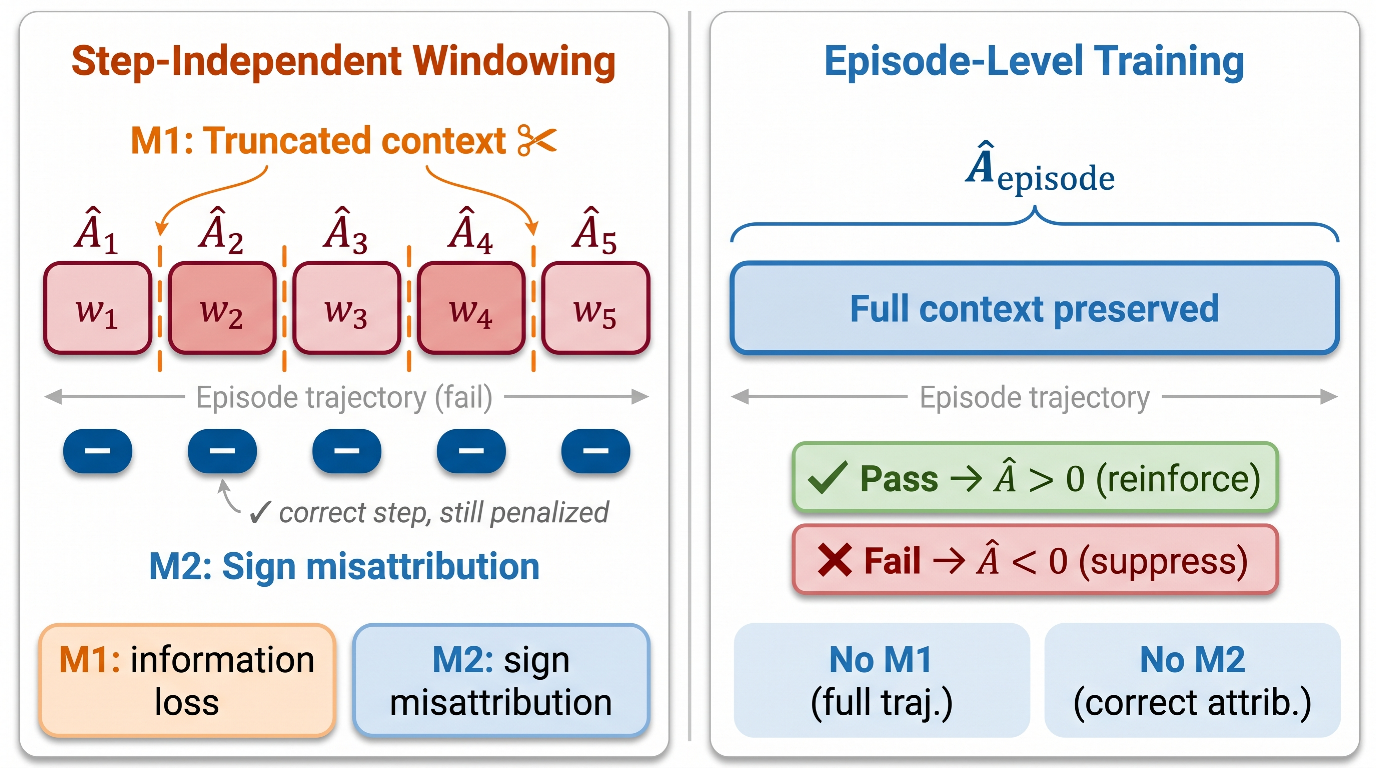
\includegraphics[width=0.85\textwidth]{fig_overview.pdf}
\caption{Step-independent windowing (left) partitions the trajectory into fixed windows, each optimized independently. This introduces two failure mechanisms: M1 (information loss) truncates context at window boundaries, and M2 (sign misattribution) assigns all windows the same advantage sign based on episode outcome. Episode-level training (right) treats the full trajectory as a single sample, eliminating both mechanisms.}
\label{fig:overview}
\end{figure*}

\section{Introduction}
\label{sec:introduction}

Reinforcement learning from sparse terminal reward has emerged as a promising paradigm for training LLM agents on multi-turn interactive tasks spanning 30--50 interaction steps~\citep{kim2025reflact,digiRL2024,wang2022scienceworld}. Group Relative Policy Optimization (GRPO)~\citep{shao2024deepseekmath}, with its critic-free design, has become the algorithm of choice. Yet a gap persists between the promise of RL-driven agent improvement and the reality of training outcomes: recent agent RL systems~\citep{ragen2025,selfguide2026,spear2025,feng2025gigpo} share a common, unscrutinized implementation pattern (decomposing trajectories into fixed-size windows, each optimized independently) and frequently report training instability without diagnosing its root cause.

We show this \textit{step-independent} default introduces a fundamental credit assignment pathology. Step-independent training partitions trajectories into non-overlapping $h$-step windows, each optimized via GRPO. This produces a two-phase collapse: task success drops to 0\% while action validity initially remains high, then continued training destroys even basic formatting. Preliminary comparisons suggest that standard remedies (dense reward shaping, discount tuning) do not resolve the pathology (Appendix~\ref{app:additional}). Concurrent methods that improve per-step credit quality (GiGPO~\citep{feng2025gigpo}, GAGPO~\citep{gagpo2026}, Turn-PPO~\citep{turnppo2025}, HCAPO~\citep{hcapo2026}) address the credit assignment challenge through improved step-level mechanisms, validating that sign correctness is the critical factor. Our contribution is orthogonal: we formally diagnose \textit{why} the default windowing fails.

We trace the collapse to two mechanisms at different layers. \textit{\textbf{Policy information loss}} (M1) operates at the inference layer: each window lacks access to earlier observations, imposing a constant performance ceiling. \textit{\textbf{Advantage sign misattribution}} (M2) operates at the training layer: under binary reward, the advantage sign reflects episode success rather than local action quality. Our theoretical analysis shows that a substantial fraction of gradient updates for locally correct actions (those contributing to episode success; Definition~1) carry incorrect sign (Section~\ref{sec:theory}), a prediction confirmed by direct measurement (Section~\ref{sec:sign_verification}). Sign errors, amplified by the M1--M2 feedback loop, cause progressive degradation rather than merely slow convergence. Our primary contribution is diagnostic: we identify, formalize, and empirically validate a previously uncharacterized pathology in the dominant training paradigm. Episode-level GRPO (restoring GRPO's original per-sample granularity to the episode level) structurally eliminates both mechanisms by treating the full trajectory as a single optimization sample, achieving substantial OOD improvement where step-independent collapses to 0\%, with preliminary evidence of persistence at 8B scale.

Our contributions:
\begin{enumerate}[nosep,leftmargin=*]
\item \textbf{Dual mechanism diagnosis.} We formalize \textit{information loss} and \textit{sign misattribution} as distinct failure modes with different temporal behaviors (constant ceiling versus cumulative degradation) and derive closed-form expressions for the probability of incorrect gradient direction.
\item \textbf{Controlled empirical separation.} A partial factorial experiment isolates each mechanism: removing sign misattribution converts collapse into bounded learning; removing information loss enables OOD generalization. Direct sign measurement confirms the theoretical prediction at near-random credit agreement (alignment between advantage sign and action quality).
\item \textbf{Systematic evaluation and generality.} Episode-level training structurally eliminates both mechanisms, but an 11-seed evaluation reveals that avoiding collapse is necessary but not sufficient: only 36\% of seeds achieve significant OOD transfer. Cross-scale (8B) and cross-environment (ScienceWorld) evidence provides preliminary support for generality.
\end{enumerate}

\section{Related Work}
\label{sec:related_work}

\paragraph{RL for multi-turn LLM agents.}
GRPO~\citep{shao2024deepseekmath}, Proximal Policy Optimization (PPO)~\citep{schulman2017ppo}, and reinforcement learning from human feedback (RLHF) methods~\citep{ouyang2022instructgpt,rafailov2023dpo} have been extended to multi-turn agents~\citep{yao2023react,ragen2025} via step-independent windowing. RAGEN~\citep{ragen2025} introduced this decomposition as a practical solution to memory constraints, partitioning trajectories into fixed-size windows each optimized as independent GRPO samples. Subsequent work builds on this foundation: DigiRL~\citep{digiRL2024} applies online RL to web agents with autonomous reward, SPEAR~\citep{spear2025} addresses entropy collapse through progressive reward scaling, and SelfGuide~\citep{selfguide2026} uses self-generated rewards. These systems inherit the step-independent design without examining its credit assignment implications. Our work identifies this shared choice as a structural failure point.

\paragraph{Credit assignment in RL.}
The credit assignment problem (determining which actions contributed to an outcome) is fundamental to RL~\citep{sutton1988td,williams1992reinforce}. Classical solutions include temporal difference learning, eligibility traces, and generalized advantage estimation~\citep{schulman2016gae} (Appendix~\ref{app:classical_connection}). Step-independent GRPO inherits the worst of outcome-vs-process supervision~\citep{lightman2024lets}: all windows receive episode-level credit regardless of individual action quality. Recent methods address this at different granularities: ArCHer~\citep{zhou2024archer} and VinePPO~\citep{kazemnejad2024vineppo} improve value estimation, PRIME~\citep{prime2025}, VAPO~\citep{vapo2025}, and iStar~\citep{istar2025} refine credit granularity, while GiGPO~\citep{feng2025gigpo}, Turn-PPO~\citep{turnppo2025}, SWEET-RL~\citep{sweetrl2025}, MT-GRPO~\citep{mtgrpo2025}, GAGPO~\citep{gagpo2026}, and HCAPO~\citep{hcapo2026} propose step- or turn-level advantage computation that preserves sign correctness. Our framework provides a unified explanation for \textit{why} these finer-grained methods succeed: they eliminate M2 (sign misattribution) while operating within the windowed framework. IRC~\citep{irc2026}, MC-GRPO~\citep{mcgrpo2026}, GRPO-$\lambda$~\citep{grpolambda2025}, OAR~\citep{oar2026}, and~\citet{gradientcoupling2025} independently corroborate our sign-level diagnosis from complementary perspectives.

\paragraph{GRPO collapse phenomena.}
Training instability under GRPO has been documented across multiple settings. RAGEN-2~\citep{ragen2_2026} and GRPO-Collapse~\citep{grpocollapse2025} report reward variance collapse where all rollouts converge to similar returns, zeroing out advantages. RC-GRPO~\citep{rcgrpo2026} and EDGE-GRPO~\citep{edgegrpo2025} propose variance-preserving modifications. Our dual-mechanism framework subsumes these observations: reward variance collapse is a special case of the reward saturation phenomenon we analyze in Section~\ref{sec:theory}, arising when $\sigma \to 0$ in GRPO normalization. The M1--M2 vicious cycle (where information loss depresses success rate, amplifying sign errors, which further degrade performance) provides a causal mechanism for the empirically observed death spirals.

\begin{figure}[t]
\centering
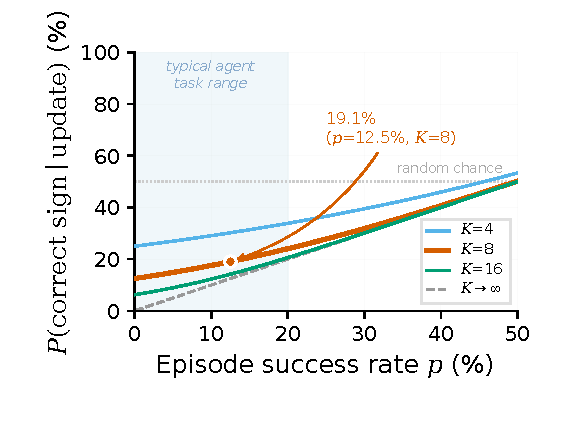
\includegraphics[width=\columnwidth]{fig_theory_curve.pdf}
\caption{Upper bound on the probability of correct gradient sign vs.\ episode success rate $p$ (Proposition~2). At typical agent task success rates ($p < 0.2$, shaded), the majority of gradient updates carry incorrect sign regardless of group size $K$.}
\label{fig:theory_curve}
\end{figure}

\section{Method}
\label{sec:method}

\subsection{Problem Formulation and GRPO}
\label{sec:problem_formulation}

We model the multi-turn agent as a partially observable Markov decision process (POMDP)~\citep{kaelbling1998planning} where the policy $\pi_\phi(a_t \mid h_t)$ generates actions conditioned on interaction history $h_t = (o_1, a_1, \ldots, o_t)$. Episodes of $T$ steps terminate with binary reward $R \in \{0, r_+\}$ (our experiments use a penalty variant with $r_- = -0.1$ per invalid action; Section~\ref{sec:setup}). GRPO~\citep{shao2024deepseekmath} samples $K$ rollouts per task and computes group-relative advantages:
\begin{align}
\hat{A}_k &= \frac{R_k - \mu}{\sigma + \epsilon}, \notag \\
\mu &= \frac{1}{K}\sum_{j=1}^K R_j, \quad \sigma = \sqrt{\frac{1}{K}\sum_{j=1}^K (R_j - \mu)^2}
\label{eq:grpo_advantage}
\end{align}
GRPO is episode-level by design: each rollout receives one return and one advantage, with no inherent temporal discounting.

\subsection{Step-Independent Windowing}
\label{sec:step_independent}

Agent RL frameworks must reconcile GRPO's episode-level design with the memory constraints of long trajectories. RAGEN~\citep{ragen2025} introduces \textbf{step-independent training}: the trajectory is partitioned into non-overlapping $h$-step windows, each receiving a discounted return:
\begin{equation}
R_w = \gamma^{(N - w)} \cdot R_{\text{episode}}
\label{eq:step_return}
\end{equation}
where $w \in \{1, \ldots, N\}$ indexes windows and $N = \lceil T/h \rceil$ is the number of windows. Each window is optimized as an independent GRPO sample. This reduces sequence length from $O(T)$ to $O(h)$ and multiplies the effective batch size, but structurally alters credit assignment.

\subsection{Dual Mechanism Analysis}
\label{sec:dual_mechanism}

Two mechanisms jointly cause training failure under step-independent optimization.

\subsubsection{Mechanism 1: Policy Information Loss}
\label{sec:m1_information_loss}

Step-independent training truncates context at both inference and training time. The policy $\pi_\phi(a_t \mid h_{\text{window}_w})$ conditions on only the local $h$-step history, losing access to earlier observations. With $h{=}2$, a window at step~8 has no access to the outcome of an exploration action at step~4, so the policy cannot learn strategies spanning more than $h$ steps. This imposes a \textit{constant} performance ceiling: no amount of optimization can recover absent information.

\subsubsection{Mechanism 2: Advantage Sign Misattribution}
\label{sec:m2_sign_misattribution}

Group normalization under step-independent training produces advantages whose sign reflects the \textit{episode} outcome, not local action quality:
\begin{equation}
\text{sign}(\hat{A}_w) \approx \text{sign}(R_{\text{episode}} - \mu)
\label{eq:sign_correlation}
\end{equation}
In failed episodes ($R_{\text{episode}} = 0$), all windows receive negative advantages when $\mu > 0$, including windows with locally correct actions. Conversely, successful episodes reinforce all windows, including those with suboptimal actions. Unlike M1's constant ceiling, sign misattribution is \textit{cumulative}: each wrong-sign gradient step further erodes policy competence. The discount factor $\gamma^{(N-w)}$ introduces magnitude decay across positions, but sign errors are strictly more harmful: magnitude decay slows convergence, while sign errors cause active divergence.

\subsection{Episode-Level Training}
\label{sec:episode_level}

Episode-level training structurally eliminates both mechanisms by treating the complete trajectory as a single GRPO sample. The full history $h_t$ is available at every step (eliminating M1), and a single advantage $\hat{A}$ applies uniformly to all tokens (eliminating M2). Uniform reinforcement of successful trajectories preserves good sub-strategies; window-level sign errors actively destroy them. This restores GRPO's original per-sample granularity to the episode level; step-independent windowing is the deviation introduced by multi-turn agent frameworks.

\subsection{Partial Factorial Design}
\label{sec:factorial_design}

To separate the two mechanisms, we design a $2 \times 2$ partial factorial varying observation scope and advantage granularity: \textbf{Cell~A} (truncated $h{=}2$ + step-level advantage; both mechanisms active), \textbf{Cell~B} (truncated $h{=}2$ + episode-level advantage; only M1 active), \textbf{Cell~D} (full trajectory + episode-level advantage; neither active), and \textbf{Cell~C} (full trajectory + step-level advantage; only M2 active). Cell~C encountered persistent numerical instability across six hyperparameter configurations (Appendix~\ref{app:cell_c}); we therefore evaluate a partial 3-of-4 factorial. Comparing A vs.\ B isolates sign misattribution; comparing B vs.\ D isolates information loss.

\begin{figure*}[t]
\centering
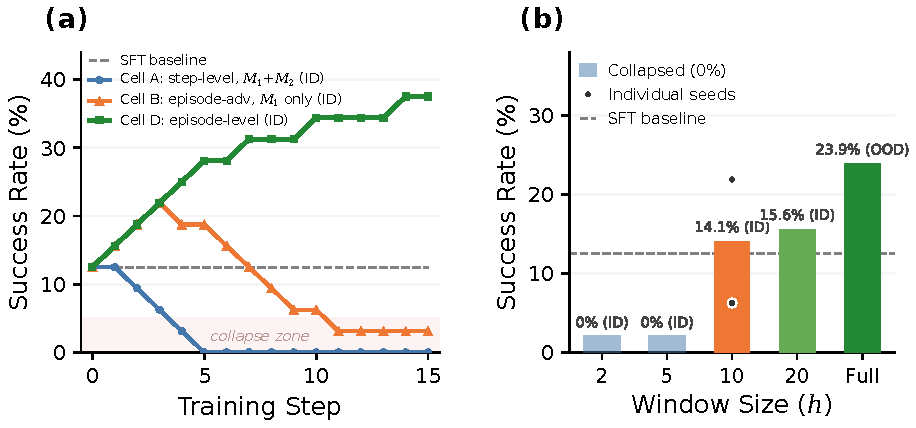
\includegraphics[width=\textwidth]{fig_training_dynamics.pdf}
\caption{(a)~Training dynamics across partial factorial conditions. Cell~A collapses; Cell~B shows bounded learning; Cell~D improves monotonically. (b)~Window size $h$ vs.\ success rate. Bars show mean over available seeds; black dots at $h{=}10$ show individual seeds (2 seeds), revealing seed-dependent instability at this boundary. Hatched bars indicate collapsed conditions ($0\%$).}
\label{fig:hsweep}
\end{figure*}

\section{Theoretical Analysis}
\label{sec:theory}

Sign misattribution is the more fundamental failure mechanism because it causes active divergence, not merely slow convergence. We derive the probability of incorrect gradient direction below; full proofs appear in Appendix~\ref{app:theory_full}.

\textbf{Definition 1} (Locally correct action). \textit{An action $a_t$ is \textbf{locally correct} if it would receive positive advantage under an oracle that observes the full episode history $h_t$ and has access to the true action-value function. Equivalently,\footnote{This equivalence is approximate; it holds exactly when all trajectories within an episode are equally likely under the reference policy, and approximately under the mild assumption that policy drift remains small during early training. This approximation is most accurate when the policy has not yet diverged significantly from initialization (here, $p \approx 12.5\%$); at higher success rates, the bound may loosen.} window $w$ contains locally correct actions if replacing them (holding all other windows fixed) would decrease the probability of episode success.}

\textbf{Proposition 1.} \textit{Under step-independent training with binary episode reward $R_{\text{episode}} \in \{0, r_+\}$, the probability that window $w$'s advantage $\hat{A}_w$ has the correct sign (aligned with local action quality) approaches the base success rate $p$ as the number of rollouts $K$ per group increases.}

\textit{Proof sketch.} In a failed episode ($R_{\text{episode}} = 0$), all windows receive $R_w = 0$. If any rollout in the group succeeded, $\mu > 0$, so every window in the failed episode receives $\hat{A}_w < 0$, including windows with locally correct actions. The probability of receiving the wrong sign in a failed episode is $1 - (1-p)^{K-1}$ (at least one group member succeeded). As $K$ grows, this approaches $1-p$, and the overall probability of correct sign approaches $p$. \hfill$\square$

The key distinction is temporal. Information loss (M1) imposes a constant ceiling determined by $h$; sign misattribution (M2) is cumulative: each wrong-sign gradient step erodes policy competence below that ceiling. A wrong-sign gradient moves the optimizer \textit{away} from good policies; a reduced-magnitude gradient from discounting ($\gamma^{(N-w)}$) still points toward good policies. Sign errors produce active divergence; magnitude errors merely slow convergence (Appendix~\ref{app:sign_fundamental}).

\textbf{Proposition 2.}\label{prop:correct_sign} \textit{Let $p$ denote the episode success rate and $K$ the number of rollouts per group. Under step-independent training with binary episode reward, the fraction of gradient updates with correct sign is upper bounded by:}
\begin{equation}
P(\text{correct} \mid \text{update}) \leq \frac{p}{1 - (1-p)^{K}}
\label{eq:correct_conditional}
\end{equation}

\textit{Derivation.} Three mutually exclusive cases determine gradient direction for a window with locally correct actions: (1)~episode succeeded (probability $p$): correct sign; (2)~episode failed but group contains a success (probability $(1{-}p)[1{-}(1{-}p)^{K-1}]$): wrong sign; (3)~entire group failed (probability $(1{-}p)^K$): zero gradient. Conditioning on non-zero gradient (Cases 1 and 2) yields Equation~\ref{eq:correct_conditional}. The bound is tight when episode success implies all constituent windows are locally correct; in practice, successful episodes may contain suboptimal windows, so the true fraction of correctly signed updates may be lower.

Proposition~2 provides a finite-sample refinement of Proposition~1's asymptotic result: while Proposition~1 establishes that the probability of correct sign converges to $p$ as $K \to \infty$, Proposition~2 gives an explicit upper bound for any finite group size $K$. At $p{=}12.5\%$, $K{=}8$, this yields an upper bound of 19.1\% on correctly signed gradient updates (Figure~\ref{fig:theory_curve}). In the large-$K$ limit, $P(\text{correct} \mid \text{update}) \to p$: ${\sim}87.5\%$ of updates for locally correct windows point in the wrong direction.

\paragraph{Severity scales with task difficulty.} Sign misattribution becomes \textit{more} severe as the task gets harder (Equation~\ref{eq:correct_conditional}): at $p{=}50\%$, $P(\text{correct} \mid \text{update}) \leq 50.2\%$; at $p{=}5\%$, at most 14.9\% of updates are correct. Multi-turn agent tasks with low baseline success rates are precisely where credit assignment matters most, yet where step-independent training produces the worst gradient signal. Increasing $K$ does not help: more updates occur (fewer all-fail groups), but each remains equally likely to carry the wrong sign.

\paragraph{Reward saturation.} When all $K$ rollouts receive the same binary reward, $\sigma = 0$ and $\hat{A}_w = 0$, producing zero gradient. At $p{=}12.5\%$, $K{=}8$, roughly one-third of batches yield no gradient ($(1{-}p)^K \approx 34.4\%$). This compounds sign misattribution: of the ${\sim}66\%$ that produce a gradient, at most 19.1\% have the correct sign.

\paragraph{Cumulative divergence.} Sign misattribution produces a systematic gradient bias. Let $\theta^*$ denote an optimal policy parameterization. At each update, the expected gradient under step-independent training is:
\begin{equation}
\mathbb{E}[\nabla_\theta \mathcal{L}] = P_c \cdot g_+ + (1 - P_c) \cdot g_-
\label{eq:biased_gradient}
\end{equation}
where $P_c = P(\text{correct} \mid \text{update})$, $g_+$ points toward $\theta^*$, and $g_-$ points away. When $P_c < 0.5$ (which holds for $p < 0.5$; Equation~\ref{eq:correct_conditional}), the expected gradient points away from good policies even if correct-sign updates carry larger magnitude: the break-even ratio is $|g_+|/|g_-| \geq (1{-}P_c)/P_c \approx 4.2$ at $p{=}12.5\%$, while the empirically measured ratio is ${\approx}2.6$ (Section~\ref{sec:sign_verification}), confirming that sign frequency dominates magnitude compensation. Amplified by the M1--M2 feedback loop (Section~\ref{sec:dual_mechanism}), this drives progressive degradation: M1 caps $p$; lower $p$ increases wrong-sign frequency under M2, further depressing $p$.

\paragraph{Extension to ternary reward.} Our experimental setting uses ternary reward ($r \in \{-0.1, 0, 1\}$) rather than binary. Under ternary reward with penalty rate $\alpha$ (fraction of actions receiving $r_-$), binary reward ($\alpha{=}0$) yields the tightest bound on sign misattribution. Increasing $\alpha$ introduces within-group variance among failed episodes that partially breaks the sign-outcome coupling: windows with valid actions in failed episodes may obtain positive advantage when penalty-induced variance shifts the group mean downward. The measured 52\% credit agreement at $\alpha{\approx}0.3$ is consistent with this monotonic relaxation from the binary worst case. A binomial test confirms that the binary upper bound (19.1\%) and the empirical rate (52.1\%) measure different quantities ($z = 45.9$, $p < 10^{-100}$); both are far below the level required for reliable policy improvement (Appendix~\ref{app:nonbinary_extension}).

\section{Experiments}
\label{sec:experiments}

Step-independent training collapses while episode-level training succeeds; a partial factorial design separates the two mechanisms; and window size $h$ modulates severity.

\subsection{Setup}
\label{sec:setup}

We evaluate on ALFWorld~\citep{shridhar2021alfworld}, a text-based household environment with six task types requiring sequential reasoning over up to 50 steps. The environment provides ternary reward ($r_- {=} {-}0.1$ per invalid action, $0$ for valid but unsuccessful, $r_+$ for success); our theory assumes simplified binary reward ($R \in \{0, r_+\}$), yielding an upper bound on sign misattribution (Section~\ref{sec:sign_verification} validates under both). The base policy is Qwen3-1.7B~\citep{qwen3_2025} fine-tuned on expert demonstrations (SFT baseline: 12.5\% in-distribution), where Proposition~2 predicts the majority of gradient updates carry incorrect sign. All conditions use RAGEN~\citep{ragen2025} (v0.1)\footnote{Our implementation extends RAGEN v0.1 with episode-level training support. Code available upon acceptance.} with GRPO~\citep{shao2024deepseekmath} ($K{=}8$; Appendix~\ref{app:hyperparameters}). We report success rate on a 134-task OOD set (primary) and 32-task in-distribution set (secondary).

\subsection{Partial Factorial Mechanism Separation}
\label{sec:factorial_experiments}

We implement the partial factorial design from Section~\ref{sec:factorial_design} (3 of 4 cells; Cell~C excluded due to NaN instability; Appendix~\ref{app:cell_c}) with two seeds per condition. Cell~C's qualitatively different failure (divergence rather than gradual collapse) suggests information loss may unintentionally stabilize gradient variance, questioning exact separability (Section~\ref{sec:discussion}).

\subsection{Results}
\label{sec:results}

Cell~A collapses in two phases (Table~\ref{tab:main_results}): task success drops to ${\leq}$3\% by step~5 and remains below 10\% through step~15, while action validity initially remains high; continued sign misattribution then destroys even basic formatting.
Cell~B eliminates sign misattribution while retaining information loss: training success improves, but OOD generalization (5.97\%) remains near the SFT baseline (6.72\%), confirming that removing M2 alone bounds learning without causing degradation.
Cell~D is the only condition that substantially exceeds the SFT baseline, with monotonic OOD improvement across both seeds.
The A$\to$B comparison isolates M2; the B$\to$D comparison isolates M1. Both mechanisms are necessary to explain the full failure pattern (Figure~\ref{fig:hsweep}a).

\begin{table}[t]
\centering
\caption{1.7B results on ALFWorld (best checkpoint per seed). Full seed-level breakdown in Table~\ref{tab:seed_variability} and Appendix~\ref{tab:additional_baselines}.}
\label{tab:main_results}
\resizebox{\columnwidth}{!}{%
\begin{tabular}{@{}llccc@{}}
\toprule
\textbf{Condition} & \textbf{Mechanisms} & \textbf{Best Step} & \textbf{In-Dist (\%)} & \textbf{OOD (\%)} \\
\midrule
SFT baseline & --- & --- & 12.50 & 6.72 \\
Cell A ($h{=}2$, step) & M1+M2 & 5 & 1.56$^\S$ & --- \\
Cell B ($h{=}2$, episode) & M1 only & 5 & 18.75 & 5.97$^\ast$ \\
Cell D (full, episode) & neither & 15 & \textbf{34.38} & \textbf{17.16} \\
\bottomrule
\end{tabular}}
\begin{flushleft}
\small $^\ast$ Single seed; seed2 best checkpoint unavailable for re-evaluation. \\
\small $^\S$ Mean of two seeds (0\% and 3.13\%); seed~1 collapses to 0\% by step~15; seed~2 shows partial recovery (9.4\%). OOD not evaluated at this checkpoint.
\end{flushleft}
\end{table}

\paragraph{Additional conditions.} Dense reward, REINFORCE++, and discount-factor sweep experiments suggest that sign misattribution, not reward sparsity or discounting, drives the failure (Appendix~\ref{app:additional}).

\paragraph{Window-size sweep.} Varying window size reveals $h{=}10$ as a seed-dependent boundary (Figure~\ref{fig:hsweep}b). Windows of $h{\leq}5$ collapse to 0\% across all seeds; $h{=}20$ and full-episode conditions recover monotonically. At $h{=}10$, two seeds diverge (6.25\% vs.\ 21.9\%, mean 14.1\%), placing this window size at the instability boundary rather than in a deterministic collapse zone. All other conditions are single-seed.
\label{sec:results_hsweep}

\subsection{Sign Misattribution Verification}
\label{sec:sign_verification}

We distinguish three metrics that each capture a different aspect of credit assignment quality:

\textit{(1) Sign-episode correlation}: whether advantage sign tracks episode outcome. Under binary reward (penalty${=}0$), correlation is near-perfect at 99.6\% ($270/271$ non-zero windows; Figure~\ref{fig:sign_misattribution}), directly confirming M2: advantage sign is determined by episode outcome, not local action quality.\footnote{The single discordant window arises from GRPO group-composition effects, not a violation of the mechanism.} This follows by construction, since all windows in a successful episode share the same positive return.

\textit{(2) Credit agreement rate}: whether advantage sign matches local action quality, operationalized via action validity as a proxy (Definition~1). Under penalty reward ($h{=}2$, $n{=}3{,}000$ windows), only 52.07\% of valid-action windows receive positive advantage ($p{=}0.025$ vs.\ 50\%; Cohen's $h \approx 0.041$, below the small-effect threshold), confirming near-random credit agreement. Under binary reward, agreement drops to 28\% ($n{=}271$), as advantage sign systematically penalizes valid actions in failed episodes. This metric is an upper bound: valid actions include strategically suboptimal moves, yet agreement remains near-random even under this generous criterion.

\textit{(3) $P(\text{correct} \mid \text{update})$}: the theoretical upper bound from Proposition~2 ($\leq$19.1\% at $p{=}12.5\%$, $K{=}8$). This bounds the fraction of non-zero gradient updates with correct sign, a different quantity from the credit agreement rate, which conditions on action validity rather than gradient participation. The two metrics are complementary: Proposition~2 bounds worst-case gradient quality; credit agreement measures empirical signal strength.

The empirical magnitude ratio $|\hat{A}_{\text{correct}}|/|\hat{A}_{\text{wrong}}| \approx 2.6$ at step~5 ($n{=}30$) falls below the break-even threshold $(1{-}P_c)/P_c \approx 4.2$, confirming magnitude asymmetry cannot compensate for sign frequency (Section~\ref{sec:theory}). Combined with $\gamma{=}1.0$ collapse (Appendix~\ref{app:additional}), these measurements support sign misattribution as a primary factor, though the credit agreement effect is small ($+$2pp).

\begin{figure}[t]
\centering
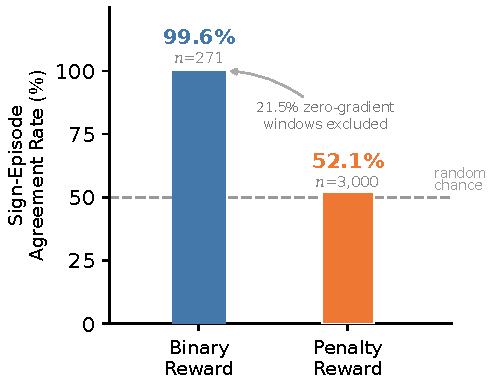
\includegraphics[width=\columnwidth]{fig_sign_misattribution.pdf}
\caption{Sign-episode correlation (binary reward) vs.\ credit agreement rate (penalty reward). Under binary reward, advantage sign tracks episode outcome near-perfectly, confirming M2. Under penalty reward, credit agreement drops to near-random chance (dashed line).}
\label{fig:sign_misattribution}
\end{figure}

\subsection{Episode-Level Training: Seed Variability}
\label{sec:seed_variability}

Episode-level GRPO addresses the dual-mechanism failure, but outcomes remain seed-dependent. We evaluate $N{=}11$ seeds under identical hyperparameters, classifying each as \textbf{collapsed} (in-distribution success declines $>$50\% from peak for $\geq$3 steps), \textbf{stagnant} (stable but not significant vs.\ SFT), or \textbf{generalized} (Fisher exact $p{<}0.01$ vs.\ SFT on the 134-task OOD set). Table~\ref{tab:seed_variability} reports best-checkpoint results per seed.

\begin{table}[t]
\centering
\caption{Episode-level GRPO across 11 seeds (134 OOD tasks, best checkpoint per seed). C=Collapsed, S=Stagnant, G=Generalized (Fisher exact $p{<}0.01$ vs.\ SFT). NS=not significant. Wilson 95\% confidence interval. SFT baseline: 6.72\%.}
\label{tab:seed_variability}
\resizebox{\columnwidth}{!}{%
\begin{tabular}{@{}llcccc@{}}
\toprule
\textbf{Seed} & \textbf{Step} & \textbf{Cat.} & \textbf{OOD (\%)} & \textbf{95\% CI} & \textbf{vs SFT} \\
\midrule
seed2048$^\ddagger$ & 5 & C & 8.21 & [4.6, 14.2] & NS \\
seed42$^\ddagger$ & 5 & C & 12.69 & [8.0, 19.4] & NS \\
seed8 & 5 & C & 11.94 & [7.5, 18.5] & NS \\
\midrule
seed200 & 5 & S & 10.45 & [6.3, 16.8] & NS \\
seed300 & 5 & S & 10.45 & [6.3, 16.8] & NS \\
seed100 & 10 & S & 12.69 & [8.0, 19.4] & NS \\
seed2$^\ddagger$ & 15 & S & 15.67 & [10.5, 22.8] & $p{=}0.03$ \\
\midrule
seed1 & 5 & G$^\dagger$ & 23.88 & [17.4, 31.8] & $p{<}0.001$ \\
seed5 & 10 & G & 29.10 & [22.1, 37.3] & $p{<}0.001$ \\
seed6 & 15 & G & 29.10 & [22.1, 37.3] & $p{<}0.001$ \\
seed4 & 15 & G & 30.60 & [23.5, 38.7] & $p{<}0.001$ \\
\bottomrule
\end{tabular}}
\begin{flushleft}
\small $^\dagger$ RAGEN built-in eval; checkpoint unavailable for re-evaluation. \\
\small $^\ddagger$ OOD evaluated via RAGEN built-in eval; not independently re-evaluated under 134-task OOD evaluation protocol. \\
\small All results are single-run evaluations at decoding temperature $\tau{=}0.4$; see Limitations for eval variance discussion.
\end{flushleft}
\end{table}

\begin{figure}[t]
\centering\vspace{-3pt}
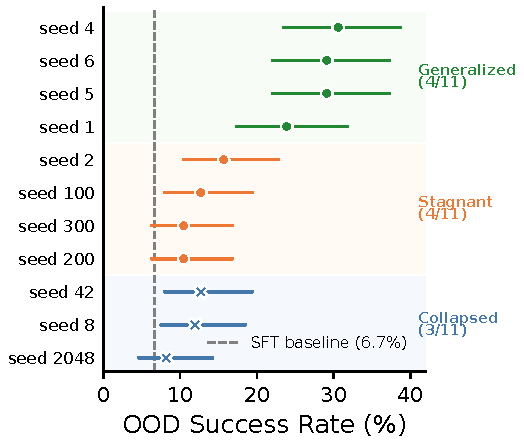
\includegraphics[width=0.95\columnwidth]{fig_seed_variability.pdf}\vspace{-5pt}
\caption{OOD success rate across 11 episode-level GRPO seeds (Wilson 95\% CI). Seeds partition into \textit{Generalized} ($p{<}0.01$ vs.\ SFT), \textit{Stagnant} (stable, NS), and \textit{Collapsed} ($\times$). Avoiding collapse is necessary but not sufficient.}
\label{fig:seed_variability}\vspace{-8pt}
\end{figure}

Three outcomes emerge (Table~\ref{tab:seed_variability}, Figure~\ref{fig:seed_variability}): ${\sim}$27\% collapse with response length inflation (Appendix~\ref{app:response_length}), ${\sim}$36\% stagnate near SFT, and ${\sim}$36\% generalize. The 11-seed mean OOD success rate is 17.7\%, compared to the SFT baseline of 6.72\%. Unified step-5 evaluation across all seeds guards against checkpoint selection bias (Appendix~\ref{app:step5_unified}). Stable training is necessary but not sufficient; the mechanism driving seed-dependent transfer remains open (Section~\ref{sec:discussion}).

\subsection{Cross-Scale and Cross-Environment Verification}
\label{sec:cross_scale}

A single-seed 8B experiment confirms both failure and fix persist at scale: Cell~A collapses within two steps while Cell~D reaches 90.3\% OOD (Appendix~\ref{app:8b_results}); restricting to $h{=}2$ confirms severe information loss. The pathology is environment-general: step-independent training on ScienceWorld~\citep{wang2022scienceworld} also collapses to 0\% across all 15 steps with comparable M1 gap.

\section{Discussion}
\label{sec:discussion}

\paragraph{Generality and mechanism interaction.}
Sign misattribution arises whenever step-level windowing, sparse binary reward, and group-relative normalization co-occur (Section~\ref{sec:theory}), though verified only on GRPO with ALFWorld and ScienceWorld. Cell~C's NaN divergence (full trajectory + step-level advantage) prevents empirical isolation of M2; our factorial interpretation assumes approximate separability, which the remaining three cells are consistent with but cannot definitively confirm. Cell~C's qualitatively different failure mode suggests M1 may unintentionally stabilize training by limiting gradient variance (Appendix~\ref{app:why_defaults}). Multi-seed evaluation reveals bimodal OOD transfer pointing to initialization sensitivity (Appendix~\ref{app:early_signal}).

\paragraph{Concurrent methods.}
HCAPO~\citep{hcapo2026} and GiGPO~\citep{feng2025gigpo} succeed with $h{=}2$ by eliminating M2 through finer-grained credit, consistent with our framework's prediction (see Limitations). We provide a practical decision guide for selecting among episode-level and step-level methods based on which mechanisms are active in a given setting (Appendix~\ref{app:method_selection}).


\section{Conclusion}
\label{sec:conclusion}

Step-independent training fails through two interacting mechanisms: information loss imposes a constant ceiling while sign misattribution causes cumulative degradation. Episode-level GRPO structurally eliminates both, though the fix is seed-dependent (36\% generalize significantly). This finding applies to GRPO-style methods under step-level windowing, sparse reward, and group-relative normalization, verified on ALFWorld and ScienceWorld.


\section*{Limitations}

Our experiments span two environments (ALFWorld, ScienceWorld) and two scales (1.7B, 8B); additional environments and scales would strengthen generality, and the 8B and ScienceWorld results are single-seed. Among 11 seeds at 1.7B, only 36\% achieve significant OOD generalization; the mechanism driving seed-dependent transfer remains open. OOD evaluations are single-run at $\tau{=}0.4$; multi-run averaging would reduce evaluation variance (Appendix~\ref{app:eval_variance}). Episode-level training increases sequence length from $O(h)$ to $O(T)$, which may limit scalability to very long episodes without further engineering. We do not reproduce concurrent methods (HCAPO, Turn-PPO, GiGPO); our framework predicts their success through finer-grained credit, consistent with published results (Section~\ref{sec:discussion}).

\bibliography{references}

\clearpage
\appendix

\section{Theoretical Analysis: Full Derivations}
\label{app:theory_full}

\subsection{Why Sign Misattribution is the Core Mechanism}
\label{app:sign_fundamental}

The two mechanisms identified in Section~\ref{sec:dual_mechanism} operate at different layers and produce qualitatively different failures. Policy information loss (Mechanism 1) operates at the inference layer, restricting the observable context and establishing a structural performance ceiling that is constant across training. Sign misattribution (Mechanism 2) operates at the training layer, corrupting gradient directions and progressively degrading performance below this ceiling.

\textit{Proof of Proposition 1.} Define ``correct sign'' as follows: for a window containing locally beneficial actions, the correct sign of $\hat{A}_w$ is positive (reinforcement); for a window containing locally detrimental actions, the correct sign is negative (suppression). Under binary reward, the return for window $w$ is $R_w = \gamma^{(N-w)} \cdot R_{\text{episode}}$ (Equation~\ref{eq:step_return}). In a failed episode ($R_{\text{episode}} = 0$), all windows receive $R_w = 0$ regardless of their local action quality. If the group contains at least one successful rollout, the group mean $\mu > 0$, and all windows in the failed episode receive negative advantages after normalization via Equation~\ref{eq:grpo_advantage}. This includes windows where the agent took locally correct actions. Now consider a window with locally correct actions. In a successful episode (probability $p$), the window receives positive $\hat{A}_w$, which is the correct sign. In a failed episode (probability $1 - p$), the window receives negative $\hat{A}_w$ whenever $\mu > 0$, which is the wrong sign. The probability that $\mu = 0$ (all $K$ rollouts in the group failed) is $(1-p)^K$, which shrinks exponentially with $K$. As $K$ grows, nearly every failed episode produces a non-zero group mean, and the window receives the wrong sign with probability approaching $1-p$. The probability of correct sign therefore approaches $p$. \hfill$\square$

The distinction between sign error and magnitude error further clarifies why Mechanism 2 is catastrophic while Mechanism 1 is merely suboptimal. The discount factor $\gamma^{(N-w)}$ in Equation~\ref{eq:step_return} introduces magnitude decay across window positions: for an episode with $T=50$ steps and $h=2$, the first window ($w=1$) retains $\gamma^{N-1} = 0.95^{24} \approx 0.29$ of the terminal window's return. This attenuation reduces the gradient magnitude for early windows but preserves the gradient direction. A gradient with correct sign and reduced magnitude produces slow convergence, a condition recoverable through longer training. A gradient with wrong sign produces active divergence: the optimization pushes the policy away from good behaviors and toward bad ones.

\subsection{Formal Probability Analysis}
\label{app:formal_probability}

\textit{Derivation of Proposition 2.} For a window with locally correct actions, the gradient direction depends on $\text{sign}(\hat{A}_w)$, which depends on whether the episode succeeded and whether the group contains any successful rollouts. Three mutually exclusive cases arise.

\textit{Case 1: Episode succeeded} (probability $p$). The window receives $R_w = \gamma^{(N-w)} \cdot r_+ > 0$. With at least one failed rollout in the group, $R_w > \mu$ after normalization, producing $\hat{A}_w > 0$.\footnote{The edge case where all $K$ rollouts succeed (probability $p^K$) is negligible at the baseline success rates considered ($p^8 < 10^{-7}$ at $p = 12.5\%$).} The gradient reinforces the window's actions. For a window with locally correct actions, this is the correct direction.

\textit{Case 2: Episode failed, group contains at least one success} (probability $(1-p)[1 - (1-p)^{K-1}]$). The window receives $R_w = 0 < \mu$, producing $\hat{A}_w < 0$. The gradient suppresses the window's actions. For a window with locally correct actions, this is the wrong direction.

\textit{Case 3: Episode failed, entire group failed} (probability $(1-p) \cdot (1-p)^{K-1} = (1-p)^{K}$). All returns are zero, so $\mu = 0$ and $\sigma = 0$. The advantage is zero, producing no gradient update.

Summing Cases~1 and~3 yields $P(\text{correct sign or no update}) = p + (1-p)^{K}$. Since only Cases~1 and~2 produce non-zero gradients, the conditional probability follows as Equation~\ref{eq:correct_conditional}.

\label{app:nonbinary_extension}
\textit{Two calibers of credit assignment failure.} Proposition~2 and the empirical credit agreement rate (Section~\ref{sec:sign_verification}) quantify different aspects of credit assignment failure under different reward structures; both confirm that advantage sign carries insufficient information about local action quality.

\textit{Binary caliber} ($P(\text{correct} \mid \text{update}) \leq 19.1\%$). Under pure binary reward $R \in \{0, r_+\}$, the GRPO advantage $\hat{A}_w = R_w - \bar{R}_g$ has its sign entirely determined by episode outcome: all windows in a successful episode receive positive advantage, all windows in a failed episode receive negative advantage whenever the group contains at least one success. This near-deterministic sign-episode mapping, confirmed empirically at 99.6\% ($270/271$ windows; Section~\ref{sec:sign_verification}), means Proposition~2's upper bound applies directly: at most 19.1\% of non-zero gradient updates carry the correct sign.

\textit{Penalty caliber} (credit agreement $= 52.1\%$). Introducing a format penalty $r_- = -0.1$ per invalid action breaks this deterministic mapping. Within a failed episode, windows with valid actions receive $R_w = 0$ while windows with invalid actions receive $R_w = -0.1h$. This intra-episode variance shifts $\bar{R}_g$ downward, allowing some valid-action windows in failed episodes to obtain $\hat{A}_w > 0$ despite overall failure. Credit agreement rises from 19.1\% to 52.1\%, but this is marginally above random chance (Cohen's $h = 0.041$, below the 0.2 small-effect threshold), carrying negligible information about local action quality.

\textit{Complementary evidence.} The two calibers capture qualitatively different failure modes: 19.1\% reflects deterministic misattribution (advantage sign systematically tracks the wrong signal), while 52.1\% reflects near-random noise (advantage sign carries almost no local information). Both are far below the level required for policy improvement. The gap between them is itself informative: it quantifies how penalty-induced variance transforms the failure mode from systematic wrong-sign to random noise, without repairing credit assignment. A binomial test rejects $H_0{:}\, P = 0.191$ ($z = 45.9$, $p < 10^{-100}$), formally confirming that the two calibers measure different quantities.

We evaluate these expressions at the empirical baseline of our experiments. At $p = 12.5\%$ and $K = 8$: $(1-p)^K = 0.875^8 \approx 0.344$, giving $P(\text{correct or no update}) \approx 0.469$. Of the 65.6\% of cases that produce a gradient update, only $P(\text{correct} \mid \text{update}) = 0.125 / 0.656 \approx 19.1\%$ have the correct sign. As $K$ increases to 16, $(1-p)^{K} \approx 0.118$, and $P(\text{correct} \mid \text{update}) \approx 14.2\%$. In the large-$K$ limit, $P(\text{correct} \mid \text{update}) \to p$, so approximately $1 - p = 87.5\%$ of all gradient updates for locally correct windows point in the wrong direction.

\subsection{Why the Community Defaults to Step-Independent Training}
\label{app:why_defaults}

If step-independent training is structurally flawed for multi-turn agents, why has it become the default? We identify six contributing factors.

\textbf{1. Context length constraints.} Smaller language models (1B to 4B parameters) typically support context lengths of 2048 to 4096 tokens. Multi-turn episodes spanning 50 or more interaction steps easily exceed these limits. Step-independent windowing is a pragmatic response to a hardware constraint, not a deliberate algorithmic choice.

\textbf{2. Token-level training inertia.} Language model training is organized around predicting the next token over fixed-length sequences. When multi-turn RL inherits this paradigm, the natural unit of optimization becomes a fixed-length window rather than a variable-length episode. The mismatch between token-level optimization and episode-level credit assignment goes unquestioned because it aligns with existing training infrastructure.

\textbf{3. Inherited framework default.} The RAGEN framework~\citep{ragen2025} implements step-independent mode as its default configuration, not as one option among alternatives. Users inherit this choice without an explicit decision point, and default configurations propagate silently through downstream projects.

\textbf{4. Memory and compute constraints.} Episode-level training requires processing $O(T)$ tokens per sequence, incurring $O(T^2)$ attention cost with full self-attention. Step-independent training reduces this to $O(h)$ tokens and $O(h^2)$ attention cost per window. The computational savings are immediate and measurable, while the credit assignment failure is subtle and deferred until training collapse occurs.

\textbf{5. Reward shaping as apparent fix.} Dense reward shaping (per-step bonuses for intermediate goals) appears to address sparse reward problems. Our dense reward experiment (Section~\ref{sec:results_dense}) reveals a different failure mode: the agent maximizes format-level rewards (action validity rises from 60\% to 97.5\%) while task success remains at 0\%. Reward shaping does not resolve sign misattribution; it creates new optimization targets that the agent can game without solving the underlying task.

\textbf{6. Absence of negative results.} When step-independent training fails, practitioners attribute the failure to insufficient hyperparameter tuning or the inherent difficulty of sparse rewards. Without published analyses that isolate the credit assignment mechanism as the root cause, the community cannot distinguish between ``this problem is hard'' and ``this training paradigm is broken for this class of problems.''

\subsection{Connection to Classical Credit Assignment}
\label{app:classical_connection}

Our findings connect to a long line of work on temporal credit assignment in reinforcement learning.

\textbf{Temporal difference learning and eligibility traces.} Sutton's TD($\lambda$)~\citep{sutton1988td} provides a spectrum of credit assignment strategies parameterized by $\lambda \in [0,1]$. At $\lambda = 0$, credit is assigned via one-step bootstrapped returns. At $\lambda = 1$, TD($\lambda$) reduces to Monte Carlo returns. Step-independent training falls below this spectrum: windows are disconnected from each other, so temporal propagation of credit does not occur.

\textbf{Generalized Advantage Estimation.} GAE($\lambda, \gamma$)~\citep{schulman2016gae} extends TD($\lambda$) with a separate discount factor. GAE(1, 1) produces undiscounted Monte Carlo returns and is equivalent to episode-level GRPO without a critic. The key difference is that GAE uses value function subtraction as the baseline, while GRPO uses group normalization.

\textbf{REINFORCE.} Williams' REINFORCE algorithm~\citep{williams1992reinforce} computes policy gradients from complete episode returns with a learned baseline $b(s)$. Episode-level GRPO is equivalent to REINFORCE where the group mean $\mu$ replaces $b(s)$ and the group standard deviation $\sigma$ provides normalization. The algorithmic structure is not new. Our contribution is the diagnosis: the community's standard adaptation of this algorithm for multi-turn LLM agents (step-independent windowing) silently breaks the credit assignment structure that REINFORCE assumes.

\textbf{Multi-agent credit assignment analogy.} Step-independent windows can be understood through cooperative multi-agent games. Each window acts as an independent ``agent'' sharing a team reward but optimized without knowledge of other windows' actions. The sign misattribution problem parallels team reward credit assignment in cooperative multi-agent RL: when the team fails, all agents receive identical penalties regardless of individual contribution. In multi-agent RL, this is a recognized problem with known solutions such as counterfactual baselines and value decomposition methods.

\section{Hyperparameters}
\label{app:hyperparameters}

\begin{table}[h]
\centering
\caption{Shared RL training hyperparameters across all conditions.}
\label{tab:hyperparameters_app}
\begin{tabular}{lc}
\toprule
Parameter & Value \\
\midrule
Group size $K$ & 8 \\
Learning rate & $1 \times 10^{-6}$ \\
KL penalty $\beta$ & 0.01 \\
Discount $\gamma$ & 0.95 \\
Invalid action penalty & 0.1 \\
Tasks per training step & 16 \\
Training steps & 15 \\
\bottomrule
\end{tabular}
\end{table}

All 1.7B experiments were conducted on 2$\times$ NVIDIA RTX PRO 6000 GPUs. Each training run (15 steps, $K{=}8$ rollouts per task, 16 tasks per step) required approximately 6--8 GPU-hours. The 11-seed evaluation totaled ${\sim}$80 GPU-hours. The 8B experiment used 4$\times$ RTX PRO 6000 with Fully Sharded Data Parallel (FSDP), requiring ${\sim}$24 GPU-hours per run. ScienceWorld experiments used the same 2-GPU setup as the 1.7B ALFWorld runs.

\paragraph{SFT baseline.} The base policy was fine-tuned on 2{,}546 expert demonstrations from the ALFWorld training split following the protocol of RAGEN~\citep{ragen2025}, using learning rate $5 \times 10^{-6}$, batch size~16, and 2 epochs.

\section{Cross-Scale and Cross-Environment Results}
\label{app:8b_results}

\begin{figure*}[t]
\centering
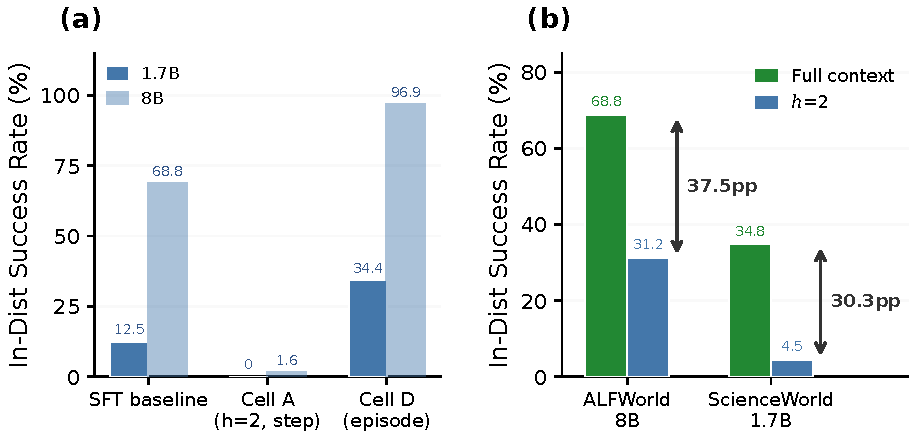
\includegraphics[width=\textwidth]{fig_cross_scale.pdf}
\caption{(a)~Cross-scale verification (single seed): both collapse (Cell~A) and fix (Cell~D) are observed from 1.7B to 8B. The episode-level fix appears more effective at 8B (96.9\% vs.\ 34.4\% in-distribution). (b)~Information loss (M1) quantification (single seed each): restricting context to $h{=}2$ drops SFT performance by 37.5pp at 8B ALFWorld and 30.3pp on ScienceWorld.}
\label{fig:cross_scale}
\end{figure*}

\begin{table}[h]
\centering
\caption{8B results on ALFWorld. SFT and $h{=}2$ use decoding temperature $\tau{=}0$; RL uses $\tau{=}0.4$. Cell~A: step~2 (post-collapse). Cell~D: step~10. Single seed. The primary comparison is Cell~A collapse (0\%) vs Cell~D success, which is independent of decoding temperature.}
\label{tab:8b_results}
\small
\begin{tabular}{@{}lcc@{}}
\toprule
\textbf{Method} & \textbf{In-Dist (\%)} & \textbf{OOD (\%)} \\
\midrule
SFT baseline & 68.75 & 80.60 \\
SFT $h{=}2$ & 31.25 & --- \\
Cell A: step-indep.\ ($h{=}2$) & 28.1 $\to$ 1.6 & --- \\
Cell D: episode-level & \textbf{96.88} & \textbf{90.30} \\
\bottomrule
\end{tabular}
\end{table}

\section{Additional Conditions}
\label{app:additional}

All conditions use single seeds unless noted.

\paragraph{Dense reward.} Step-independent $h{=}2$ with $+0.15$ per valid action. Action validity rises from 60\% to 97.5\% while task success remains 0\%; the agent games format-level rewards without solving tasks (Figure~\ref{fig:additional_conditions}b).
\label{sec:results_dense}

\paragraph{REINFORCE++.} Episode-level with per-token running-mean baseline (no critic). REINFORCE++ matches the SFT baseline (12.50\%) without improvement, suggesting that per-token advantage normalization alone does not help when the per-token baseline lacks a learned value function. This is a preliminary comparison over 15 training steps; we cannot conclude that REINFORCE++ would fail with longer training or different hyperparameters. The result suggests that naive algorithm substitution without addressing M1/M2 is insufficient, but a definitive comparison would require matched compute budgets and hyperparameter sweeps. OOD evaluation was not conducted as REINFORCE++ showed no improvement over SFT on the in-distribution set.

\begin{table}[h]
\centering
\caption{Additional baselines on ALFWorld (1.7B). Neither method improves over the SFT baseline on in-distribution tasks.}
\label{tab:additional_baselines}
\small
\begin{tabular}{@{}lccc@{}}
\toprule
\textbf{Method} & \textbf{Best Step} & \textbf{In-Dist (\%)} & \textbf{OOD (\%)} \\
\midrule
SFT baseline & --- & 12.50 & 6.72 \\
Dense reward ($h{=}2$) & 5 & 0 & 0 \\
REINFORCE++ & 5 & 12.50 & --- \\
\bottomrule
\end{tabular}
\end{table}

\paragraph{Discount factor sweep.} $\gamma \in \{0.50, 0.80, 0.95, 1.00\}$ at $h{=}5$. All four collapse to 0\% within 5 steps, including $\gamma{=}1.0$ where no magnitude decay exists. This confirms sign misattribution, not discounting, is the operative mechanism (Figure~\ref{fig:additional_conditions}a).

\begin{figure*}[t]
\centering
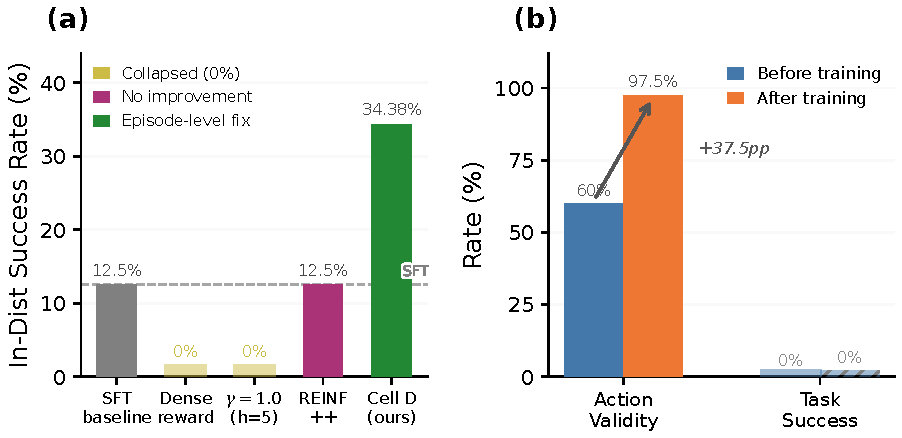
\includegraphics[width=\textwidth]{fig_additional_conditions.pdf}
\caption{(a)~Standard remedies for step-independent training: dense reward shaping and discount factor $\gamma{=}1.0$ both collapse to 0\%; REINFORCE++ matches the SFT baseline without improvement. Only episode-level training (Cell~D) exceeds baseline. (b)~Dense reward gaming: action validity rises from 60\% to 97.5\% while task success remains 0\%; the agent maximizes format-level rewards without solving tasks.}
\label{fig:additional_conditions}
\end{figure*}

\paragraph{Cell~C attempt.}
\label{app:cell_c}
Cell~C (full observation + step-level advantage) would isolate M2 without M1. We attempted this configuration across six training runs with varying hyperparameters (KL penalty $\beta \in \{0.001, 0.01, 0.04\}$, learning rate $\in \{5{\times}10^{-7}, 10^{-6}\}$). All runs terminated due to training instability: KL divergence spiked above 10.0 within 2--3 steps, triggering NaN losses. We attribute this to the combination of full-length sequences ($>$4096 tokens) with step-level advantage normalization, which produces extreme advantage magnitudes at early window positions. Cell~C remains an important gap in the partial factorial; addressing it likely requires architectural changes (e.g., gradient clipping per window position) beyond the scope of this diagnostic study.


\section{Method Selection Guide}
\label{app:method_selection}

The M1/M2 diagnostic framework guides practitioners toward the appropriate fix without exhaustive ablation. If only M2 is active (sign misattribution with sufficient observation context, e.g., $h$ large enough to preserve task-relevant information), per-step credit methods (Turn-PPO~\citep{turnppo2025}, HCAPO~\citep{hcapo2026}, GiGPO~\citep{feng2025gigpo}) directly address the failure mode. If only M1 is active (information loss without sign corruption), increasing $h$ or switching to full-context encoding suffices. When both co-occur (the typical default configuration), episode-level methods address both simultaneously. Finer-grained credit methods should be applied only after establishing an episode-level baseline, as they assume correct gradient direction.

\section{Response Length During Training}
\label{app:response_length}

\begin{figure}[h]
\centering
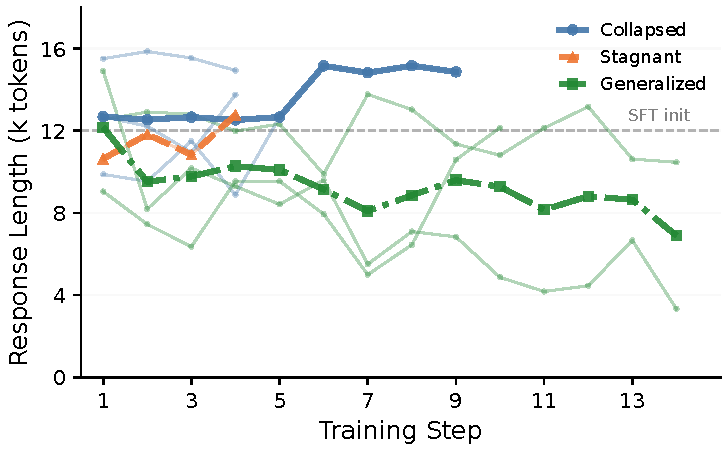
\includegraphics[width=\columnwidth]{fig_response_length.pdf}
\caption{Response length over training for 7 seeds under episode-level GRPO. Collapsed seeds (red) exhibit length inflation to 14{,}000--16{,}000 tokens. Generalized seeds (green) maintain or reduce response length. Stagnant seed (orange, seed100) remains near the SFT initialization.}
\label{fig:response_length}
\end{figure}

\section{Unified Step-5 Evaluation}
\label{app:step5_unified}

To guard against cherry-picking of checkpoints, Table~\ref{tab:step5_unified} reports all 11 seeds at a fixed evaluation point (training step~5). OOD results are included only for seeds with checkpoints evaluated under our 134-task OOD evaluation protocol (Section~\ref{sec:setup}); remaining checkpoints were unavailable for post-hoc OOD evaluation.

\begin{table}[h]
\centering
\caption{Episode-level GRPO: all 11 seeds at training step~5 (134 OOD tasks, 32 ID tasks, $\tau{=}0.4$). SFT baseline: 12.5\% ID, 6.72\% OOD. OOD results marked ``---'' indicate checkpoints unavailable for post-hoc evaluation on the 134-task OOD set. ID results marked ``---'' indicate step-5 validation metrics not recorded in training logs.}
\label{tab:step5_unified}
\small
\setlength{\tabcolsep}{4pt}
\begin{tabular}{@{}lcccc@{}}
\toprule
\textbf{Seed} & \textbf{Cat.} & \textbf{ID} & \textbf{OOD} & \textbf{vs SFT} \\
\midrule
seed2048 & C & --- & 8.21 & NS \\
seed8 & C & 28.13 & 11.94 & NS \\
seed42 & C & 9.38 & 12.69 & NS \\
\midrule
seed200 & S & --- & 10.45 & NS \\
seed300 & S & 25.00 & 10.45 & NS \\
seed100 & S & 31.25 & 11.19 & NS \\
seed2 & S & --- & --- & --- \\
\midrule
seed1 & G$^\dagger$ & --- & 23.88 & $p{<}0.001$ \\
seed4 & G & --- & --- & --- \\
seed5 & G & --- & --- & --- \\
seed6 & G & 21.88$^\ddagger$ & --- & --- \\
\bottomrule
\end{tabular}
\begin{flushleft}
\small $^\dagger$ RAGEN built-in eval; checkpoint unavailable for re-evaluation. \\
\small $^\ddagger$ Registry value 21.9\% (7/32); rounded to 21.88\% for consistency with 32-task denominator.
\end{flushleft}
\end{table}

\section{Evaluation Variance Analysis}
\label{app:eval_variance}

To quantify evaluation noise at $\tau{=}0.4$, we evaluate a single checkpoint (seed200, step~5) three times independently on the 134-task OOD set with different random seeds.

\begin{table}[h]
\centering
\caption{Evaluation variance for a single checkpoint (seed200 step~5, 134 OOD tasks, $\tau{=}0.4$). Three independent runs yield std$=$1.29pp, an order of magnitude smaller than the inter-seed performance range in Table~\ref{tab:seed_variability} (8.2\%--30.6\%).}
\label{tab:eval_variance}
\small
\setlength{\tabcolsep}{3pt}
\begin{tabular}{@{}lcccc@{}}
\toprule
\textbf{Checkpoint} & \textbf{Runs} & \textbf{OOD (\%)} & \textbf{Std} & \textbf{Range} \\
\midrule
seed200 step~5 & 3 & 11.94 & 1.29 & 2.24 \\
\bottomrule
\end{tabular}
\end{table}

The small standard deviation (1.29pp) confirms that the large inter-seed differences observed in Table~\ref{tab:seed_variability}, ranging from 8.2\% (collapsed) to 30.6\% (generalized), reflect genuine training dynamics rather than evaluation noise. We note that this variance estimate is based on a stagnant seed (seed200); generalized seeds with higher success rates may exhibit different variance profiles due to the non-linear relationship between success rate and binomial variance.

The classification threshold between stagnant and generalized seeds is based on Fisher's exact test at $p < 0.01$ vs.\ the SFT baseline; shifting to $p < 0.05$ would reclassify seed2 (the marginal case at $p = 0.03$) as generalized, changing the generalization rate from 36\% to 45\%.

\paragraph{Training efficiency.} Episode-level training processes the same total tokens as step-independent training but in fewer, longer sequences. On our hardware (2$\times$ RTX PRO 6000, 1.7B model), step-independent training ($h{=}2$) completes 15 steps in approximately 10--12 hours; episode-level training takes comparable wall-clock time as the increased sequence length is offset by fewer padding tokens.

\section{Early Training Signal Analysis}
\label{app:early_signal}

We investigated whether early training signals (steps 1--3) can predict seed-level generalization outcomes. We analyze 12 seeds grouped into three outcome categories following the definitions in Section~\ref{sec:seed_variability}: Generalized ($n{=}4$), Stagnant ($n{=}4$), and Collapsed ($n{=}4$, including seed7, which received a subsequent KL penalty intervention and is excluded from Table~\ref{tab:seed_variability}; its pre-intervention training trajectory is used here). No standard training metric (reward, KL divergence, entropy, gradient norm, response length, or train success rate) showed statistically significant between-group differences in the first three training steps (all Welch $t$-test $p > 0.2$, $n = 4$ per group). Two of the four Collapsed seeds (seed7, seed8) exhibited among the \textit{highest} early rewards and train success rates, with their collapse manifesting only after step~5 through response length inflation or reward degradation.

The strongest candidate predictor was the mutual information diversity estimate at step~1, which showed a large effect size (Cohen's $d = 1.11$) favoring Generalized over Collapsed seeds and a trending correlation with final OOD performance (Spearman $\rho = 0.43$, $p = 0.19$), but remained non-significant with the available sample size ($n = 4$ per group). These results suggest that seed-dependent outcomes are governed by mechanisms not captured by standard early training diagnostics, and that early stopping or seed selection based on initial step metrics would be unreliable.

\section{Use of AI Assistance}
We used Claude for coding, code drafting, debugging, and language polishing.


\end{document}
